\documentclass[a4paper]{article}
%\VignetteIndexEntry{Short manual for the chemCal package}
\usepackage{hyperref}

\title{Basic calibration functions for analytical chemistry}
\author{Johannes Ranke}

\usepackage{/usr/share/R/share/texmf/Sweave}
\begin{document}
\maketitle

The \texttt{chemCal} package was first designed in the course of a lecture and lab
course on "analytics of organic trace contaminants" at the University of Bremen
from October to December 2004. In the fall 2005, an email exchange with 
Ron Wehrens led to the belief that it would be desirable to implement the
inverse prediction method given in \cite{massart97} since it also covers the
case of weighted regression. Studies of the IUPAC orange book and of DIN 32645
as well as publications by Currie and the Analytical Method Committee of the 
Royal Society of Chemistry and a nice paper by Castillo and Castells provided
further understanding of the matter.

At the moment, the package consists of four functions, working on univariate
linear models of class \texttt{lm} or \texttt{rlm}, plus to datasets for
validation.

A \href{http://bugs.r-project.org/cgi-bin/R/wishlst-fulfilled?id=8877;user=guest}{bug
report (PR\#8877)} and the following e-mail exchange on the r-devel mailing list about
prediction intervals from weighted regression entailed some further studies
on this subject. However, I did not encounter any proof or explanation of the
formula cited below yet, so I can't really confirm that Massart's method is correct.

When calibrating an analytical method, the first task is to generate a suitable
model. If we want to use the \texttt{chemCal} functions, we will have to restrict
ourselves to univariate, possibly weighted, linear regression so far.

Once such a model has been created, the calibration can be graphically
shown by using the \texttt{calplot} function:

\begin{Schunk}
\begin{Sinput}
> library(chemCal)
> data(massart97ex3)
> m0 <- lm(y ~ x, data = massart97ex3)
> calplot(m0)
\end{Sinput}
\end{Schunk}
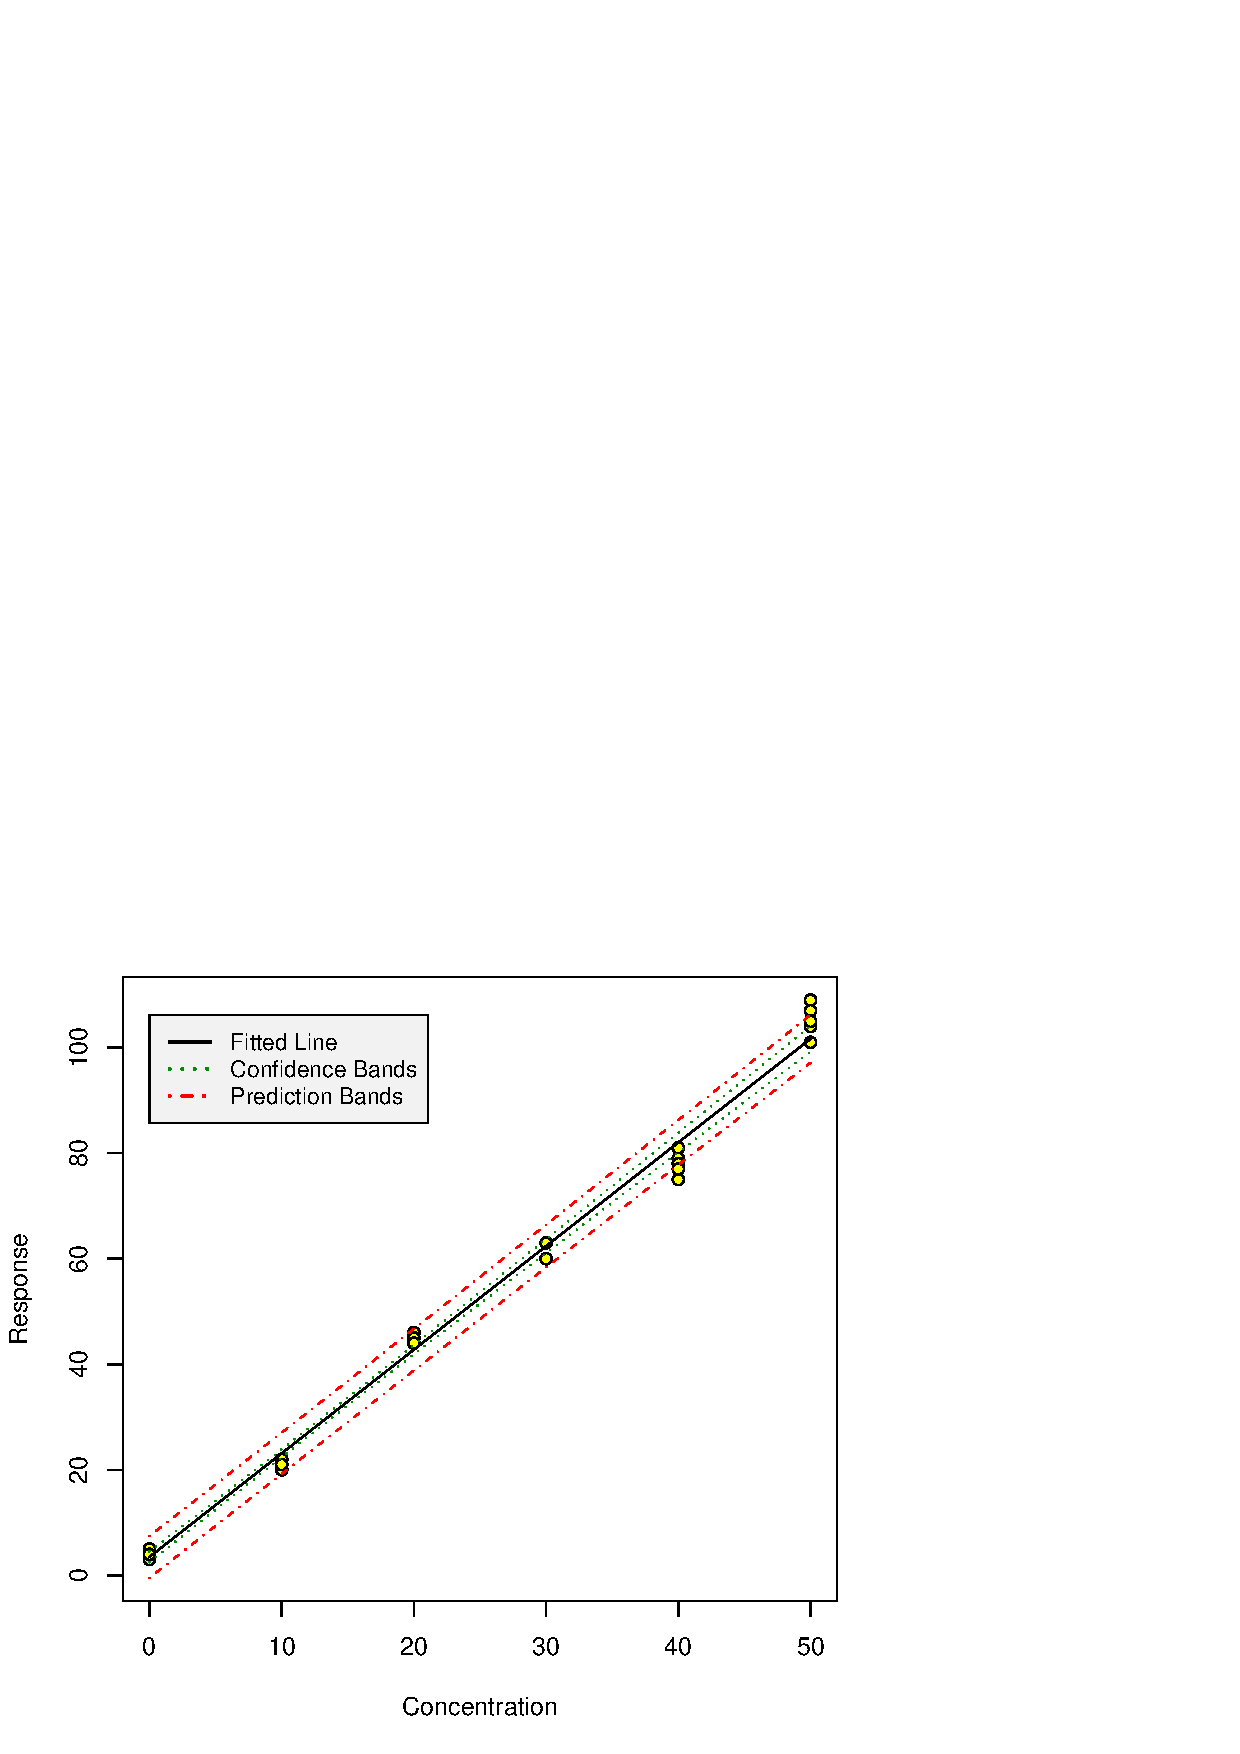
\includegraphics{chemCal-001}

As we can see, the scatter increases with increasing x. This is also
illustrated by one of the diagnostic plots for linear models 
provided by R: 

\begin{Schunk}
\begin{Sinput}
> plot(m0, which = 3)
\end{Sinput}
\end{Schunk}
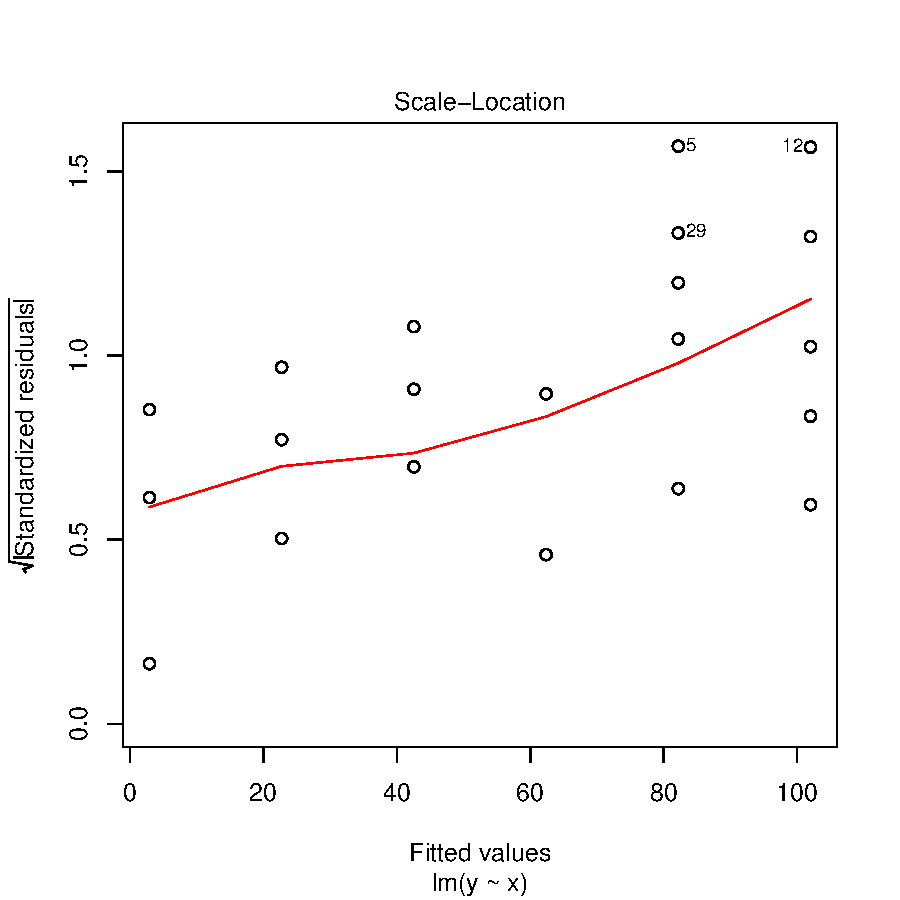
\includegraphics{chemCal-002}

Therefore, in Example 8 in \cite{massart97} weighted regression
is proposed which can be reproduced by

\begin{Schunk}
\begin{Sinput}
> attach(massart97ex3)
> yx <- split(y, x)
> ybar <- sapply(yx, mean)
> s <- round(sapply(yx, sd), digits = 2)
> w <- round(1/(s^2), digits = 3)
> weights <- w[factor(x)]
> m <- lm(y ~ x, w = weights)
\end{Sinput}
\end{Schunk}

If we now want to predict a new x value from measured y values,
we use the \texttt{inverse.predict} function:

\begin{Schunk}
\begin{Sinput}
> inverse.predict(m, 15, ws = 1.67)
\end{Sinput}
\begin{Soutput}
$Prediction
[1] 5.865367

$`Standard Error`
[1] 0.892611

$Confidence
[1] 2.478285

$`Confidence Limits`
[1] 3.387082 8.343652
\end{Soutput}
\begin{Sinput}
> inverse.predict(m, 90, ws = 0.145)
\end{Sinput}
\begin{Soutput}
$Prediction
[1] 44.06025

$`Standard Error`
[1] 2.829162

$Confidence
[1] 7.855012

$`Confidence Limits`
[1] 36.20523 51.91526
\end{Soutput}
\end{Schunk}

The weight \texttt{ws} assigned to the measured y value has to be 
given by the user in the case of weighted regression, or alternatively,
the approximate variance \texttt{var.s} at this location.

\section*{Theory for \texttt{inverse.predict}}
Equation 8.28 in \cite{massart97} gives a general equation for predicting the
standard error $s_{\hat{x_s}}$ for an x value predicted from measurements of y
according to the linear calibration function $ y = b_0 + b_1 \cdot x$:

\begin{equation}
s_{\hat{x_s}} = \frac{s_e}{b_1} \sqrt{\frac{1}{w_s m} + \frac{1}{\sum{w_i}} +
    \frac{(\bar{y_s} - \bar{y_w})^2 \sum{w_i}}
        {{b_1}^2 \left( \sum{w_i} \sum{w_i {x_i}^2} - 
            {\left( \sum{ w_i x_i } \right)}^2 \right) }}
\end{equation}

with

\begin{equation}
s_e = \sqrt{ \frac{\sum w_i (y_i - \hat{y_i})^2}{n - 2}}
\end{equation}

where $w_i$ is the weight for calibration standard $i$, $y_i$ is the mean $y$
value (!) observed for standard $i$, $\hat{y_i}$ is the estimated value for
standard $i$, $n$ is the number calibration standards, $w_s$ is the weight
attributed to the sample $s$, $m$ is the number of replicate measurements of
sample $s$, $\bar{y_s}$ is the mean response for the sample, 
$\bar{y_w} = \frac{\sum{w_i y_i}}{\sum{w_i}}$ is the weighted mean of responses
$y_i$, and $x_i$ is the given $x$ value for standard $i$.

The weight $w_s$ for the sample should be estimated or calculated in accordance
to the weights used in the linear regression. 

I adjusted the above equation in order to be able to take a different
precisions in standards and samples into account. In analogy to Equation 8.26
from \cite{massart97} we get

\begin{equation}
s_{\hat{x_s}} = \frac{1}{b_1} \sqrt{\frac{{s_s}^2}{w_s m} + 
    {s_e}^2 \left( \frac{1}{\sum{w_i}} +
        \frac{(\bar{y_s} - \bar{y_w})^2 \sum{w_i}}
            {{b_1}^2 \left( \sum{w_i} \sum{w_i {x_i}^2} - {\left( \sum{ w_i x_i } \right)}^2 \right) } \right) }
\end{equation}

where I interpret $\frac{{s_s}^2}{w_s}$ as an estimator of the variance at location
$\hat{x_s}$, which can be replaced by a user-specified value using the argument
\texttt{var.s} of the function \texttt{inverse.predict}.

\begin{thebibliography}{1}
\bibitem{massart97}
Massart, L.M, Vandenginste, B.G.M., Buydens, L.M.C., De Jong, S., Lewi, P.J.,
Smeyers-Verbeke, J. 
\newblock Handbook of Chemometrics and Qualimetrics: Part A,
\newblock Elsevier, Amsterdam, 1997
\end{thebibliography}

\end{document}
